\chapter{Controller Evaluation}
\label{chap:controller_evaluation}
% -------------------------------------------
This chapter presents the three main scenarios used to test the algorithms. The primary purpose is to evaluate the efficiency and viability of the system in adverse conditions. In addition, in a simulated way, it seeks to demonstrate that the algorithms work. Later in the annex \ref{AnexoA}, the same tests will be shown in a real test environment. Each scenario studied and the evaluation criteria used to evaluate each controller are explained below.


\section{Testing Scenarios. }


We implement three main scenarios; the first is selected to see how each agent works in a selfish environment to achieve its goal. The second tests how well the whole group can avoid an obstacle. They have to synchronize with each other and avoid obstacles without changing their goals. Moreover, the third one is selected to see how the controller works by changing the environment variables restricting the scenario and seeing how it will deal with this situation.

\subsection{ Unrestricted Highway Scenario.}


In the first scenario, we consider a highway scenario with $L$ lanes and $N$ number of vehicles driven parallel. They can be in front, behind, or to the sides. Each vehicle follows its own goal. Mainly in this scenario, there are no restrictions or obstructions.

\begin{figure}[H]
\centering
    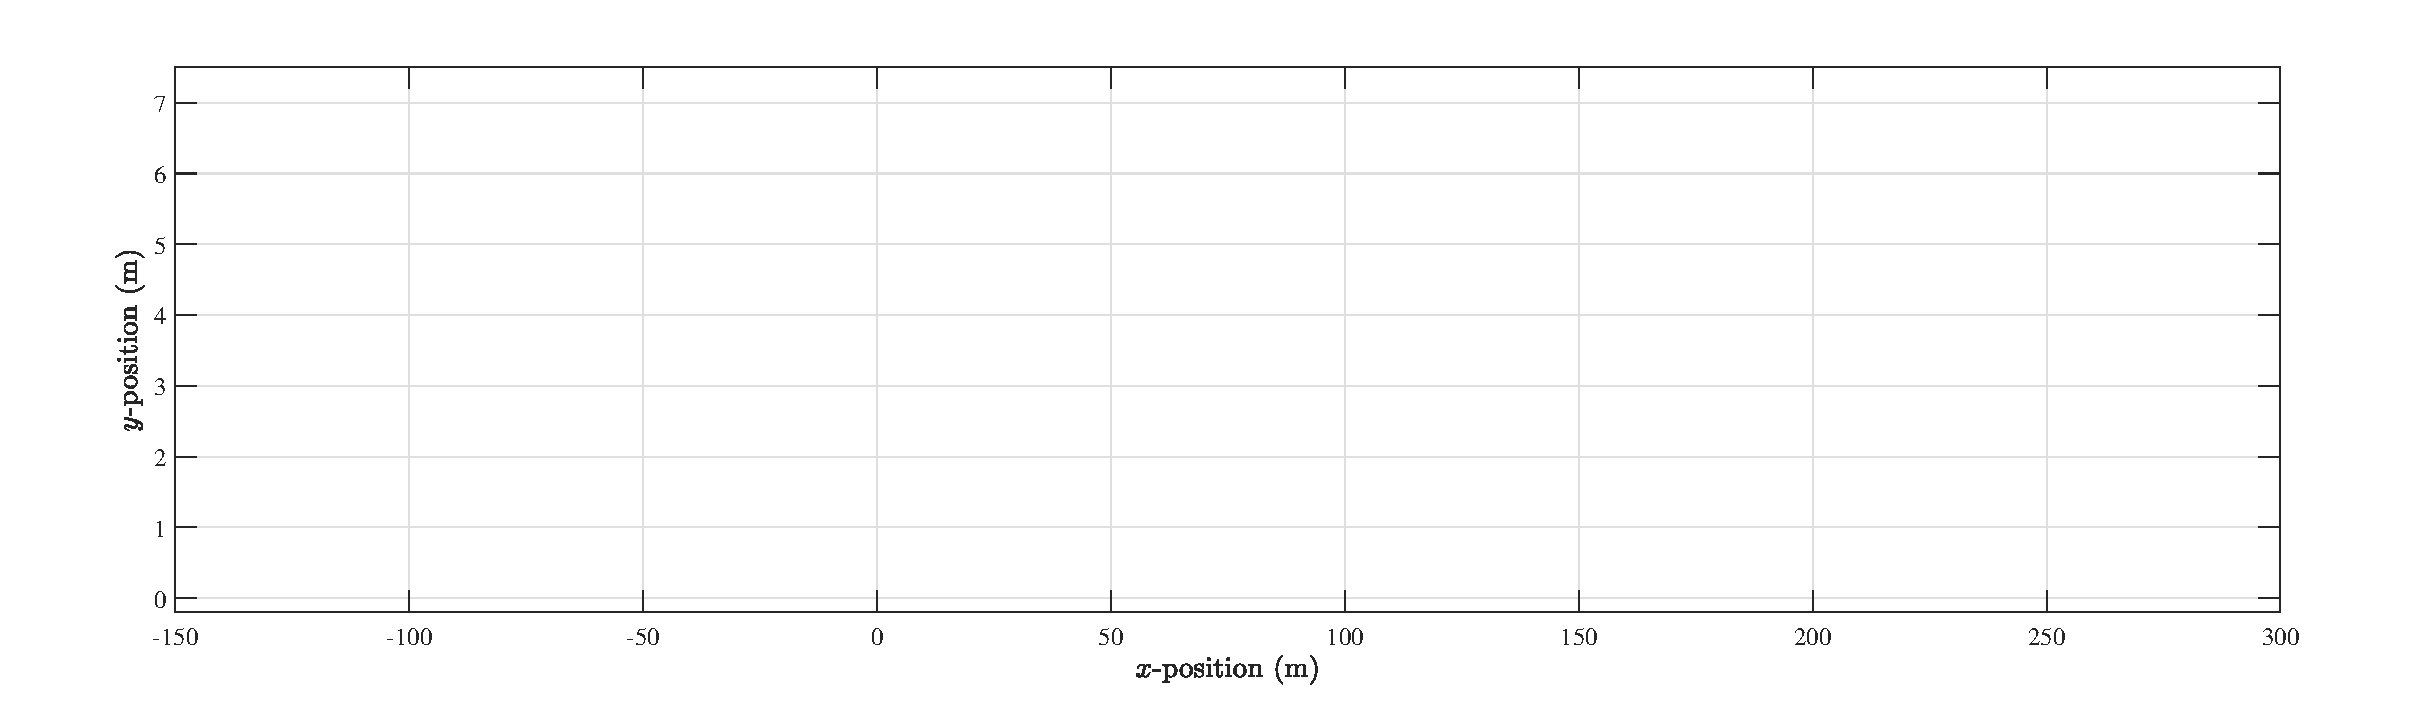
\includegraphics[width=\textwidth]{Kap5/no_restricted_scenario.eps}
    \caption{Unrestricted Scenario.}
    % \label{kinematic2}

\end{figure}


\subsection{ Obstacle Avoidance Scenario.}


In the Obstacle Avoidance Scenario, we consider the previous scenario with the same name of lanes and vehicles. Moreover, it also has an obstacle represented as a broken-down car in the middle of the road. The high-level system can detect the position of vehicles and variables in the environment. Thus a possible obstacle is a slow-moving or broken-down car.

\begin{figure}[H]
\centering
    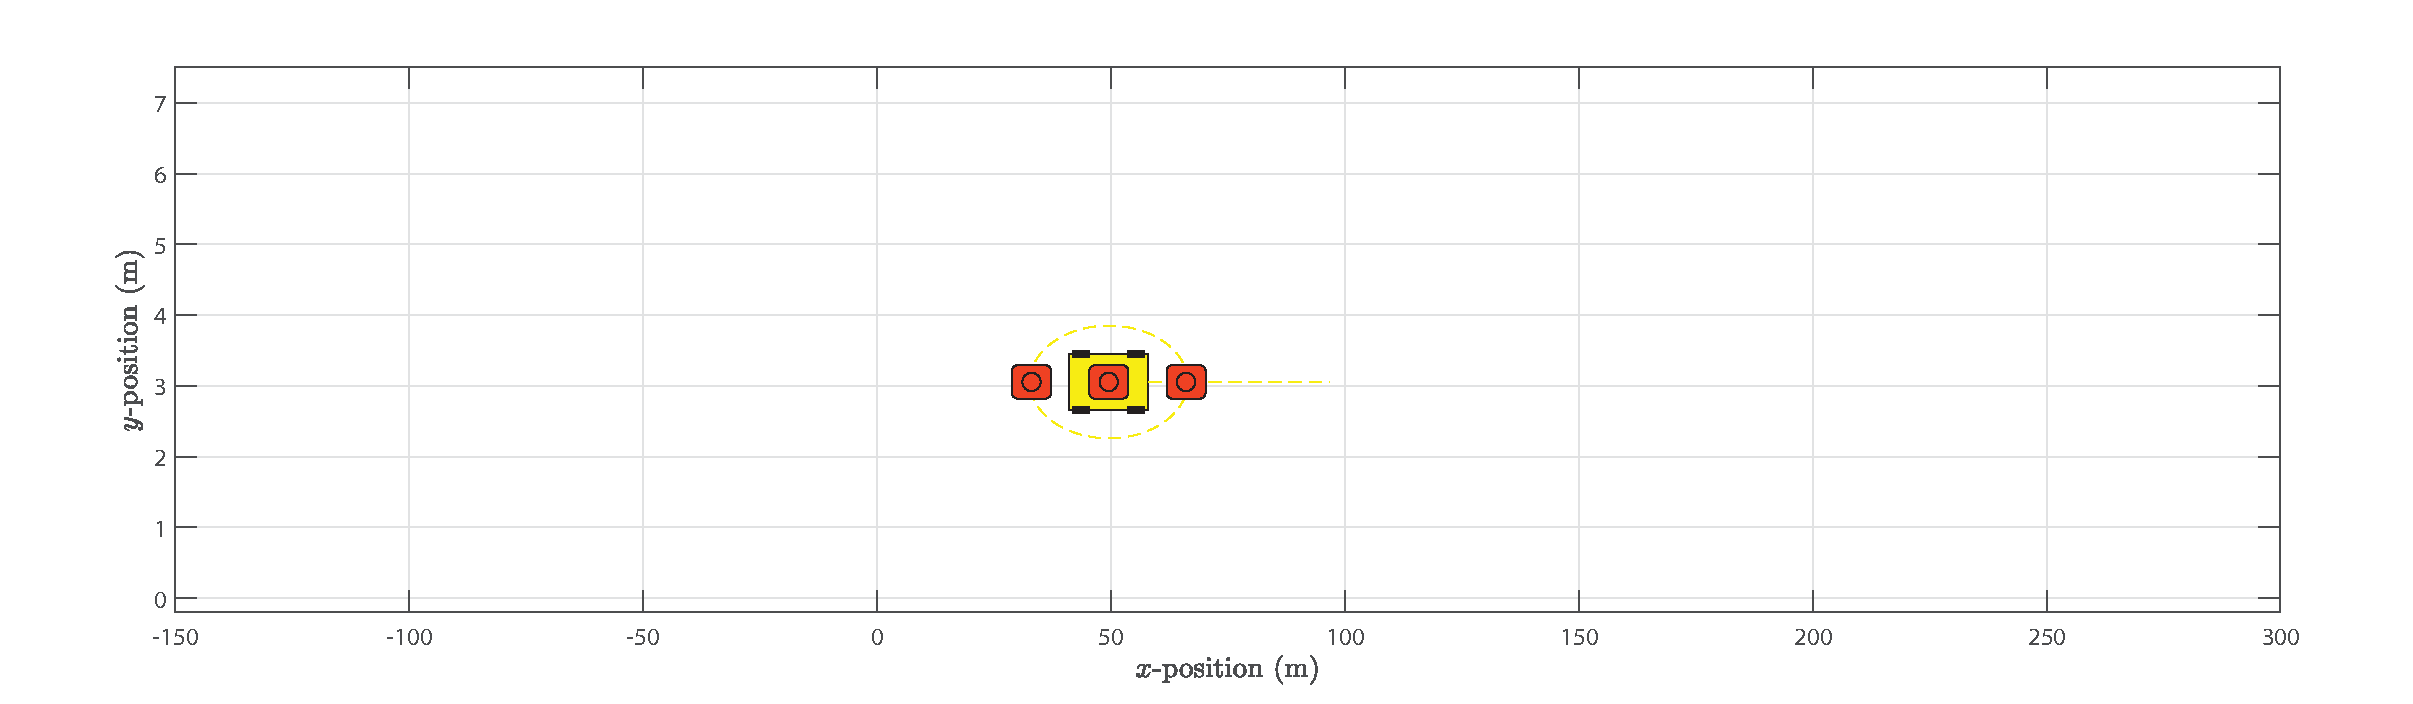
\includegraphics[width=\textwidth]{Kap5/obs_avoid_scenario.eps}
    \caption{Obstacle Avoidance Scenario.}
    % \label{kinematic2}

\end{figure}


\subsection{ Reduced Lane Scenario.}


In the restricted scenario, we consider a restriction of the environment variables. Due to work on the road, the highway is reduced to the third lane, going from 5 lanes to 1. Each vehicle will have to slow down and synchronize to be able to share a single lane. The main idea of this scenario is to check how the system behaves in the face of an aggressive variation of the environment variables.

\begin{figure}[H]
\centering
    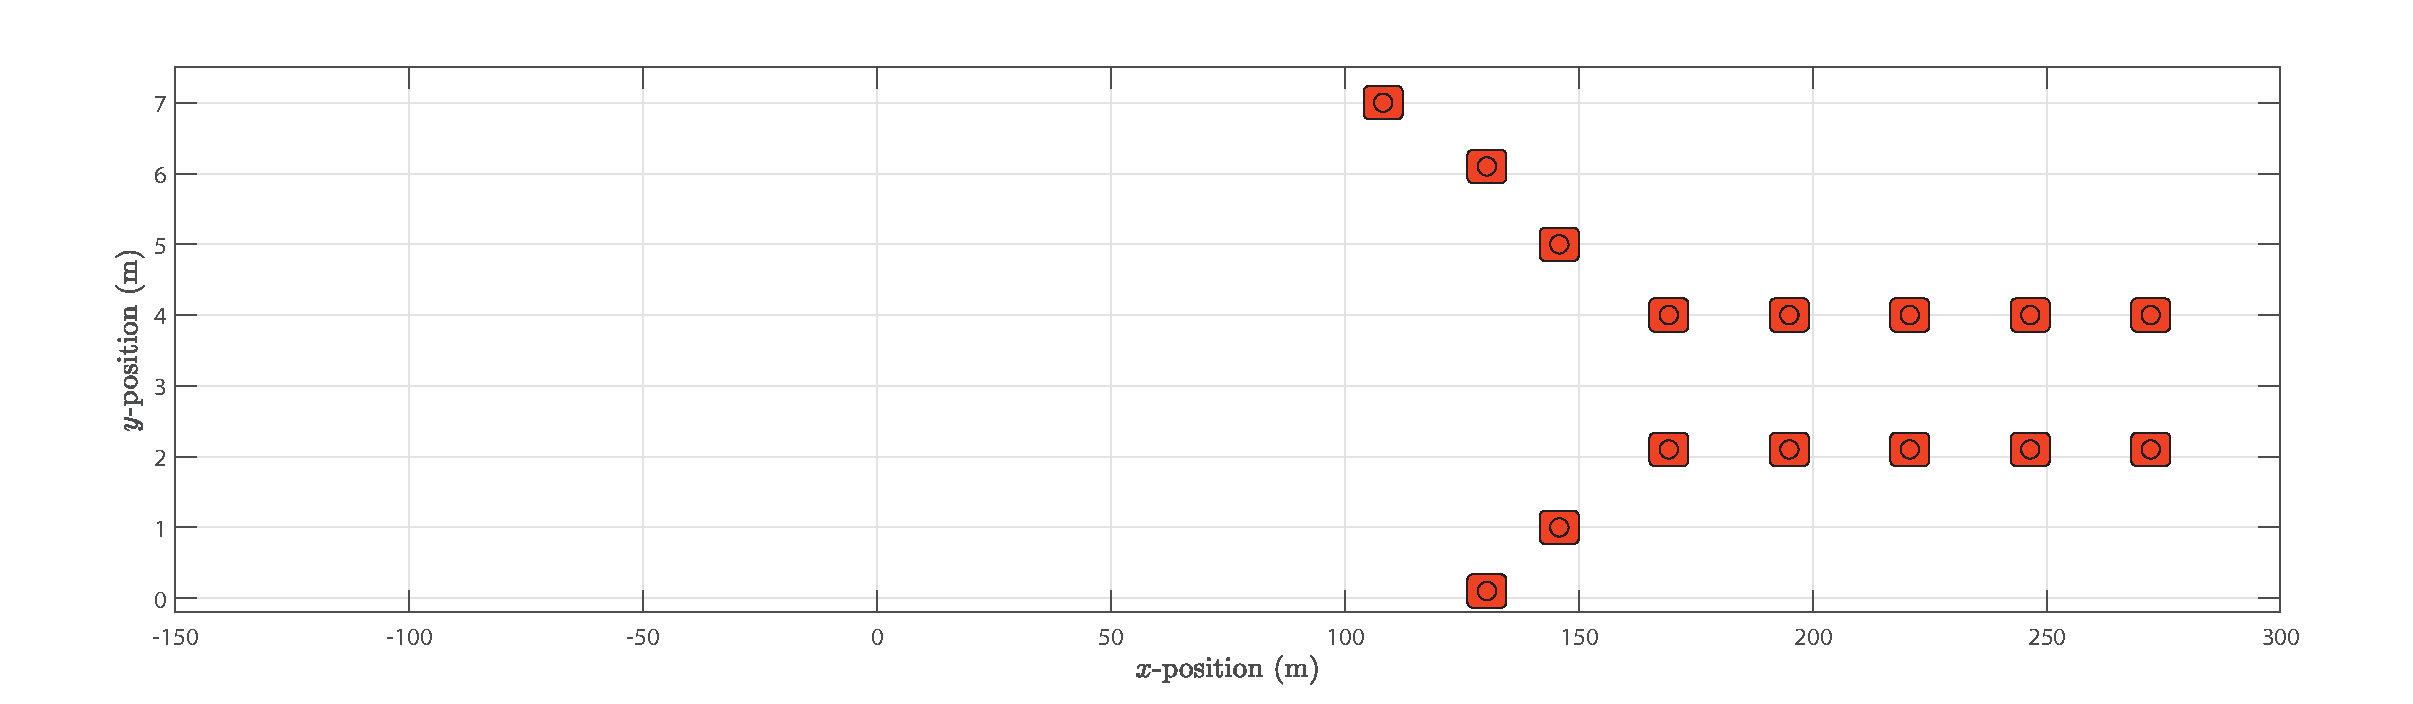
\includegraphics[width=\textwidth]{Kap5/red_lane_scenario.eps}
    \caption{Reduced Lane scenario.}
    % \label{kinematic2}
\end{figure}


\section{Evaluation Criteria.}

The controller's effectiveness and the possible strategies' feasibility established the evaluation criterion. Effectiveness focuses on the quality of the trajectory and how each agent achieves its goal. Further, feasibility focuses on the computation time and the algorithm's synchronization with the other agent's controllers.

\subsection{Feasibility}
Feasibility is one of the most essential qualities in an interconnected vehicle control system. The controller must find a control response within the sampling time. Security will be compromised if the response time is greater. We seek to obtain an algorithm with a response as fast as possible. However, the response is as accurate as possible.


\subsubsection{Computation Time. }

Computation time is crucial for the feasibility analysis of a control algorithm. A critical aspect of implementing the MPC algorithm is the sample time. The most important requirement is that the control variable's value is found within the sampling time. In centralized systems, the increase in control agents increases computing time exponentially. In decentralized systems, the computation time is held regardless of the number of agents; therefore, the following equation must be maintained: $ T_{sol} \le h$. where T-sol is the solution time it takes for the entire system to sample, and $h$ is the sampling time.

\\
The computation time is evaluated by computing the mean, max, and min over the entire simulation time.


\subsubsection{Robustness to Hardware Failure. }
Robustness is the second most important aspect of autonomous vehicle driving. A central node makes control decisions for all agents in centralized control networks. When there are connection problems, the agents cannot act due to the lack of a control signal. Each agent calculates its control response in distributed networks with information from its environment. If there are connection or communication problems, agents can still make decisions without having information about their neighbours.
\\
\\
The proposed system is decentralized; each agent receives information from its environment, finds the optimal solution in the solution space, and calculates the best control signal given the present conditions.
It is sought through the simulations to see the system's robustness in the face of disconnections, network variations, and aggressive and selfish maneuvers of its neighbours.

% \subsubsection{Trajectory Quality. }





